\chapter{Results\label{chap:result}}

    In this chapter we present the results of experiments conducted and provide answers to all research questions from Section~\ref{sec:RQs}. Section~\ref{sec:results_rq1} takes up the majority of this chapter and will be addressing results achieved on the task of \emph{Expertise Extraction}. Analysis results of \emph{Cross-Platform Expertise} will be presented in Section~\ref{sec:results_rq2}, while \emph{Cross-Platform Transferable Knowledge} results will be addressed in Section~\ref{sec:results_rq3}. This chapter will conclude with Section~\ref{sec:results_rq4}, in which we will present our results and conclusions for \emph{Expertise Evolution}.

    \section{Expertise Extraction\label{sec:results_rq1}}
        % RQ1: How to extract the major expertise areas of Stack Overflow and GitHub users? How do expertise trends compare on Stack Overflow and GitHub?
        
        For the \emph{Expertise Extraction} task \emph{3 novel techniques} have been proposed: Topic Distribution based Expertise Extraction \emph{(Technique 1)}, Expertise Extraction using LDA based User and Topic Embeddings \emph{(Technique 2)}, and Expertise Extraction using Pre-trained Word2Vec based User and Topic Embeddings \emph{(Technique 3)}. Techniques 2 and 3 have two different variations each: the first one using \emph{Average-pooling}, while the second one using \emph{Max-pooling} technique for down-sampling. Including these two variations, a total of 5 models are considered:
        
        \begin{itemize}
            \item Model 1: Topic Distribution based Expertise Extraction, labelled in tables as \textbf{TDistr}
            \item Model 2: Expertise Extraction using LDA based User and Topic Embeddings obtained by Average-pooling, labelled in tables as \textbf{LDA\_AVG}
            \item Model 3: Expertise Extraction using LDA based User and Topic Embeddings obtained by Max-pooling, labelled in tables as \textbf{LDA\_MAX}
            \item Model 4: Expertise Extraction using Pre-trained Word2Vec based User and Topic Embeddings obtained by Average-pooling, labelled in tables as \textbf{W2V\_AVG} 
            \item Model 5: Expertise Extraction using Pre-trained Word2Vec based User and Topic Embeddings obtained by Max-pooling, labelled in tables as \textbf{W2V\_AVG} 
        \end{itemize}
        
        The above listed 5 models are evaluated against a baseline (naive) model (see Section~\ref{subsec:random_model}), which is a frequency based random model. When evaluating the extraction of expertise areas, two similar experiments were used. In the first experiment each model's performance is evaluated against the ground truth knowledge from section \ref{sec:expertise_survey} with the specification that a model has to output exactly as many expertise terms as the ground truth annotation contains. This case is referred to as \emph{Experiment 1}. In the second experiment each model is evaluated against the ground truth annotation, but there are no restrictions applied to the number of expertise terms to be returned by each model. In this scenario the models can be more robust, as they can return all the expertise terms found by the underlying algorithm, without needing to rank and return only the top-$n$ expertise terms. Throughout this chapter this more robust, less restrictive experiment setup will be referred to as \emph{Experiment 2}. Furthermore, each one of the above mentioned experiments has to variations: expertise extraction from i.) GitHub data (labelled \emph{Experiment} \textbf{A}) and ii.) Stack Overflow data (labelled \emph{Experiment} \textbf{B}). 
        
        Table~\ref{tab:GH_results1} shows the top-$3$ highest evaluation metric scores for each one of the 5 models from \emph{Experiment 1A} - Expertise Extraction from GitHub Data. The top-$3$ ranking is done based on the highest \emph{Cosine Similarity} scores. The 5 models are compared against a frequency based random model (referred to as \emph{Baseline}), whose evaluation metrics comes from averaging the results of 10,000 random samples.
        
        \begin{table}
          \centering
          \caption{Results of Experiment 1A - Expertise Extraction from GitHub Data}\label{tab:GH_results1}
            \vspace{6pt} % Required to get proper spacing between caption and table
            \resizebox{\textwidth}{!}{
          \begin{tabular}{|c|c|c|c|c|c|c|c|}
            \hline
            \thead{Top 3\\Results}& \diaghead{\theadfont DiagonalHead}{Metrics}{Model} &
            \thead{\textbf{TDistr}} & \thead{\textbf{LDA\_AVG}} & \thead{\textbf{LDA\_MAX}} & \thead{\textbf{W2V\_AVG}} & \thead{\textbf{W2V\_MAX}} & \thead{\textbf{Baseline}}\\
            \hline
            \multirow{3}*{1} & Cosine Sim. & 0.6690 & 0.7187 & 0.7357 & \textbf{0.7998} & 0.7317 & 0.5962 \\
                  & Jaccard Sim. & 0.0658 & 0.0751 & 0.1040 & 0.0765 & 0.1049 & 0.0286 \\
                  & BLEU Score & 0.1197 & 0.1340 & 0.1767 & 0.1368 & 0.1782 & 0.0540 \\
            \hline
            \multirow{3}*{2} & Cosine Sim. & 0.6689 & 0.7183 & 0.7351 & 0.7959 & 0.7316 & 0.5962 \\
                   & Jaccard Sim. & 0.0658 & 0.0750 & 0.1037 & 0.0818 & 0.1049 & 0.0286 \\
                   & BLEU Score & 0.1197 & 0.1338 & 0.1762 & 0.1452 & 0.1782 & 0.0540 \\
            \hline
            \multirow{3}*{3} & Cosine Sim. & 0.6683 & 0.7183 & 0.7351 & 0.7959 & 0.7316 & 0.5962 \\
                   & Jaccard Sim. & 0.0652 & 0.0750 & 0.1037 & 0.0818 & 0.1049 & 0.0286 \\
                   & BLEU Score & 0.1186 & 0.1338 & 0.1762 & 0.1452 & 0.1782 & 0.0540 \\
          \hline 
        \end{tabular}}
        \end{table}
        
        The results from Table~\ref{tab:GH_results1} indicate very clearly that each model's top-$3$ highest evaluation scores out-perform the baseline model's each one of the three metrics. \textbf{W2V\_AVG}, which is named Expertise Extraction using Pre-trained Word2Vec based User and Topic Embeddings obtained by Average-pooling achieves the highest \emph{Cosine Similarity} score (\textbf{0.7998}), thus it can be considered the superior technique on the GitHub data set. The baseline \emph{Cosine Similarity} score of the baseline, random model is \textbf{0.5962}. \emph{Jaccard Similarity} and \emph{BLEU Score} are also reported, but \emph{Cosine Similarity} is considered the primary evaluation metric when comparing different techniques' performance, due to the reasons explained in Section~\ref{sec:eval_expertise_prediction}. \textbf{TDistr} is performing the worst, having its best \emph{Cosine Similarity} score of \textbf{0.6690}, and that is expected, since it is a topic probability distribution based technique, and does not use User and Topic Embeddings. \textbf{LDA\_MAX} and \textbf{W2V\_MAX} are performing very similarly, both plateauing around a \emph{Cosine Similarity} score of \textbf{0.73}. \textbf{LDA\_AVG} performs a little worse than  \textbf{LDA\_MAX} and \textbf{W2V\_MAX} by having the maximum \emph{Cosine Similarity} score of \textbf{0.7187}. It is difficult to understand how accurate these techniques are only based on \emph{Cosine Similarity} scores obtained from calculating the semantic similarity between the bag of words of human annotations and model extraction. To illustrate different levels of semantic similarity of \emph{Cosine Similarity} scores Table~\ref{tab:cos_sim} contains examples of word-pairs and their respective \emph{Cosine Similarity} scores. These \emph{Cosine Similarity} scores were obtained using the same pre-trained Word2Vec model\cite{efstathiou2018word} used in Section \ref{word2vec_model}. 
        
         \begin{table}
              \centering
              \caption{Example of Cosine Similarity Scores between Word-Pairs} \label{tab:cos_sim}
                \vspace{6pt} % Required to get proper spacing between caption and table
                \resizebox{\textwidth}{!}{
              \begin{tabular}{|c c c|c c c|}
                \hline
                Word 1 & Word 2 & Cosine Similarity & Word 1 & Word 2 & Cosine Similarity \\
                \hline
                php & python & 0.2529 & html & javascript & 0.6024 \\
                java & python & 0.3929 & ajax & jquery & 0.6315 \\
                analysis & visualization & 0.4524 & sklearn & tensorflow & 0.6858 \\ 
                nodejs & reactjs & 0.4909 & bagging & randomforest & 0.7251 \\
                java & jdk& 0.5517 & mysql & postgresql & 0.7997 \\
                xml & json & 0.5866 & keras & tensorflow & 0.8391 \\
                \hline
              \end{tabular}}
        \end{table}
            
        Based on the sample \emph{Cosine Similarity} scores from Table~\ref{tab:cos_sim} one can say that \textbf{W2V\_AVG}'s best model extracts expertise terms with similar semantic similarity level to the contextual similarity between the 'mysql' and 'postgresql' word-pair. Likewise, \textbf{LDA\_AVG}, \textbf{LDA\_MAX} and \textbf{W2V\_MAX} extract expertise terms with similar semantic similarity level to 'randomforest' and 'bagging' word-pair, while \textbf{TDistr}'s best \emph{Cosine Similarity} score classifies its semantic similarity level just below 'tensorflow' and 'sklearn' word-pair's. One could argue that the above mentioned semantic similarity levels correspond to contextually similar software engineering related word associations, thus illustrating that Table~\ref{tab:GH_results1}'s results lead to high levels of semantic similarity between the bags of words of human annotations and expertise terms extracted by the models. Unfortunately as far as we are aware the same kind of representation of similarity levels can not be easily created for \emph{Jaccard Similarities} and \emph{BLEU Scores}. \emph{Jaccard Similarity} is a measure of set similarity, and it highly depends not only on the magnitude of set intersection, but set union as well. \emph{BLEU Score} values range between 0 and 1, and the inventors of \emph{BLEU Score} report that in their study a professional human translator was able to achieve a score of \emph{0.3468} calculated against four reference annotations and \emph{0.2571} against two references annotations\cite{papineni2002bleu}.
        
        Table~\ref{tab:GH_params1} present in the Appendix \ref{appendix:model_params} contains all major parameters used to fit the models outlined in Table~\ref{tab:GH_results1}. The models were fitted using a hyper-parameter optimization process described in Section~\ref{sec:hyper-parameter_selection} and their parameters come from the parameter search space defined in the above mentioned Section. Table~\ref{tab:GH_params1} suggests a general pattern of the GitHub data containing a relatively small number of topics: 10 in \textbf{LDA\_AVG}, 11 being the most popular in \textbf{TDistr}, \textbf{LDA\_MAX} \& \textbf{W2V\_MAX}, and 16 in the superior \textbf{W2V\_AVG}. The parameter $\beta$ highly varies between 0.001, 0.005, 0.01 and 0.05, but in most cases $\beta=0.005$.
        
        Table~\ref{tab:SO_results1} shows the top-$3$ highest evaluation metric scores for each one of the 5 models from \emph{Experiment 1B} - Expertise Extraction from Stack Overflow Data. Same as before, the top-$3$ models are ranked based on the highest \emph{Cosine Similarity} scores, and the models are compared against a \emph{Baseline}.
        
        \begin{table}
          \centering
          \caption{Results of Experiment 1B - Expertise Extraction from Stack Overflow Data} \label{tab:SO_results1}
            \vspace{6pt} % Required to get proper spacing between caption and table
            \resizebox{\textwidth}{!}{
          \begin{tabular}{|c|c|c|c|c|c|c|c|}
            \hline
            \thead{Top 3\\Results}& \diaghead{\theadfont DiagonalHead}{Metrics}{Model} &
            \thead{\textbf{TDistr}} & \thead{\textbf{LDA\_AVG}} & \thead{\textbf{LDA\_MAX}} & \thead{\textbf{W2V\_AVG}} & \thead{\textbf{W2V\_MAX}} & \thead{\textbf{Baseline}}\\
            \hline
            \multirow{3}*{1} & Cosine Sim. & 0.5044 & 0.5582 & \textbf{0.5837} & 0.5607 & 0.5820 & 0.3721 \\
                  & Jaccard Sim. & 0.0160 & 0.0406 & 0.0435 & 0.0320 & 0.0556 & 0.0104 \\
                  & BLEU Score & 0.0313 & 0.0770 & 0.0823 & 0.0612 & 0.1041 & 0.0199 \\
            \hline
            \multirow{3}*{2} & Cosine Sim. & 0.4997 & 0.5560 & 0.5717 & 0.5574 & 0.5746 & 0.3721 \\
                  & Jaccard Sim. & 0.0295 & 0.0747 & 0.0814 & 0.0404 & 0.0784 & 0.0104 \\
                  & BLEU Score & 0.0560 & 0.1366 & 0.1471 & 0.0768 & 0.1424 & 0.0199 \\
            \hline
            \multirow{3}*{3} & Cosine Sim. & 0.4755 & 0.5409 & 0.5676 & 0.5537 & 0.5736 & 0.3721 \\
                  & Jaccard Sim. & 0.0127 & 0.0754 & 0.0821 & 0.0718 & 0.0305 & 0.0104 \\
                  & BLEU Score & 0.0247 & 0.1366 & 0.1478 & 0.1312 & 0.0584 & 0.0199 \\
          \hline 
        \end{tabular}}
        \end{table}
        
        The results from Table~\ref{tab:SO_results1} show that each model's top-$3$ highest evaluation scores out-perform the baseline model on each one of the three metrics. \textbf{LDA\_MAX}, which is named Expertise Extraction using LDA based User and Topic Embeddings obtained by Max-pooling achieves the highest \emph{Cosine Similarity} score (\textbf{0.5837}) thus it can be considered the superior technique on the Stack Overflow data set. The baseline \emph{Cosine Similarity} score of the baseline, random model is \textbf{0.3721}, which is much lower than all other model's \emph{Cosine Similarity} scores. \textbf{TDistr} is performing the worst, having its best \emph{Cosine Similarity} score of \textbf{0.5044}. \textbf{LDA\_AVG} and \textbf{W2V\_AVG} are performing very similarly, both plateauing close to a \emph{Cosine Similarity} score of \textbf{0.56}. \textbf{W2V\_MAX} is a very close second by having a maximum \emph{Cosine Similarity} score of \textbf{0.5820}, and barely being outperformed by the superior \textbf{LDA\_MAX}. The results of Table~\ref{tab:SO_results1} clearly show a trend of \textbf{LDA\_MAX} and \textbf{W2V\_MAX} outperforming \textbf{LDA\_AVG} and \textbf{W2V\_AVG}. This means that performing down-sampling using Max-pooling, instead of Average-pooling seems to work better on the Stack Overflow data set, which was not necessarily the case in Experiment 1A conducted on the GitHub data set.
        
        Sample \emph{Cosine Similarity} scores from Table~\ref{tab:cos_sim} can help associate semantic similarity levels to the results presented in Table~\ref{tab:SO_results1}. Based on Table~\ref{tab:cos_sim} one can say that  \textbf{LDA\_MAX} and \textbf{W2V\_MAX}'s best models extract expertise terms with similar semantic similarity level to the contextual similarity between the 'xml' and 'json' word-pair. Likewise, \textbf{LDA\_AVG} and \textbf{W2V\_AVG} extract expertise terms with similar semantic similarity level to 'java' and 'jdk' word-pair, while \textbf{TDistr}'s best \emph{Cosine Similarity} score classifies its semantic similarity level just above 'nodejs' and 'reactjs' word-pair's. The above mentioned word-pairs correspond to contextually similar software engineering related word associations with similar semantic similarity levels to the model performances in Table~\ref{tab:SO_results1}, thus one could argue that Table~\ref{tab:SO_results1}'s results lead to high levels of semantic similarity between the bags of words of human annotations and expertise terms extracted by the models.
        
        Table~\ref{tab:SO_params1} present in the Appendix \ref{appendix:model_params} contains all major parameters used to fit the models outlined in Table~\ref{tab:SO_results1}. Table~\ref{tab:SO_params1} suggests a general pattern of the GitHub data containing a relatively large number of topics: \{40,29,45\} in  \textbf{TDistr}, and \textbf{LDA\_AVG} and \textbf{LDA\_MAX} have 33 \& 27 number of topics in common, while \textbf{W2V\_AVG} and \textbf{W2V\_MAX} have 48 \& 31 number of topics in common. The most common number of topics out of the best performing models is 27. The parameter $\beta$ highly varies between 0.01, 0.1, 0.5 and 1, but in most cases $\beta=1$.
        
        \begin{table}
          \centering
          \caption{Results of Experiment 2A - Expertise Extraction from GitHub Data}\label{tab:GH_results2}
            \vspace{6pt} % Required to get proper spacing between caption and table
            \resizebox{\textwidth}{!}{
          \begin{tabular}{|c|c|c|c|c|c|c|c|}
            \hline
            \thead{Top 3\\Results}& \diaghead{\theadfont DiagonalHead}{Metrics}{Model} &
            \thead{\textbf{TDistr}} & \thead{\textbf{LDA\_AVG}} & \thead{\textbf{LDA\_MAX}} & \thead{\textbf{W2V\_AVG}} & \thead{\textbf{W2V\_MAX}} & \thead{\textbf{Baseline}}\\
            \hline
            \multirow{3}*{1} & Cosine Sim. & 0.6828 & 0.7377 & 0.7602 &  &  & 0.5962 \\
                  & Jaccard Sim. & 0.0246 & 0.0218 & 0.0251 &  &  &  0.0286 \\
                  & BLEU Score & 0.0277 & 0.0245 & 0.0279 &  &  &  0.0540 \\
            \hline
            \multirow{3}*{2} & Cosine Sim. & 0.6827 & 0.7364 & 0.7598 &  &  & 0.5962 \\
                   & Jaccard Sim. & 0.0249 & 0.0256 & 0.0254 &  &  & 0.0286 \\
                   & BLEU Score & 0.0281 & 0.0292 & 0.0288 &  &  &  0.0540 \\
            \hline
            \multirow{3}*{3} & Cosine Sim. & 0.6821 & 0.7362 & 0.7595 &  &  & 0.5962 \\
                   & Jaccard Sim. & 0.0241 & 0.0244 & 0.0259 &  &  & 0.0286 \\
                   & BLEU Score & 0.0271 & 0.0278 & 0.0295 &  &  &  0.0540 \\
          \hline 
        \end{tabular}}
        \end{table}
        
        
        \begin{table}
          \centering
          \caption{Results of Experiment 2B - Expertise Extraction from Stack Overflow Data} \label{tab:SO_results2}
            \vspace{6pt} % Required to get proper spacing between caption and table
            \resizebox{\textwidth}{!}{
          \begin{tabular}{|c|c|c|c|c|c|c|c|}
            \hline
            \thead{Top 3\\Results}& \diaghead{\theadfont DiagonalHead}{Metrics}{Model} &
            \thead{\textbf{TDistr}} & \thead{\textbf{LDA\_AVG}} & \thead{\textbf{LDA\_MAX}} & \thead{\textbf{W2V\_AVG}} & \thead{\textbf{W2V\_MAX}} & \thead{\textbf{Baseline}}\\
            \hline
            \multirow{3}*{1} & Cosine Sim. & 0.5263 &  & 0.5837 &  &  & 0.3721 \\
                  & Jaccard Sim. & 0.0099 &  & 0.0435 &  &  & 0.0104 \\
                  & BLEU Score & 0.0117 &  & 0.0822 &  &  & 0.0199 \\
            \hline
            \multirow{3}*{2} & Cosine Sim. & 0.5080 &  & 0.5717 &  &  & 0.3721 \\
                  & Jaccard Sim. & 0.0223 &  & 0.0816 &  &  & 0.0104 \\
                  & BLEU Score & 0.0267 &  & 0.1471 &  &  &  0.0199 \\
            \hline
            \multirow{3}*{3} & Cosine Sim. & 0.5036 &  & 0.5697 &  &  & 0.3721 \\
                  & Jaccard Sim. & 0.0111 &  & 0.0303 &  &  & 0.0104 \\
                  & BLEU Score & 0.0136 &  & 0.0579 &  &  & 0.0199 \\
          \hline 
        \end{tabular}}
        \end{table}
        
        \begin{table}
          \centering
          \caption{Examples} \label{tab:expertise_extractions}
            \vspace{6pt} % Required to get proper spacing between caption and table
             \resizebox{\textwidth}{!}{
            \begin{tabular}{|p{2cm}|p{5cm}|p{5cm}|p{1cm}|p{1cm}|}
                \hline
                Example Type & Human Annotation & Model Extraction & Match & Cosine Sim.\\
                \hline
                Bad & X & Y & 1 & 0  \\
                Mediocre & [tls, programming, oss\_fuzz, c, bcyrpt, go, security, ssl, \textbf{rust}, \textbf{java}, homebrew, urllib3, \textbf{python}, software\_engineering, objective\_c, \textbf{ruby}, azure, powershell, \textbf{shell}, infra, propery\_base\_testing, cryptography, networking, makefile, html, open\_ssl, cpython, algorithms, \textbf{clojure}, vorbis]  & [\textbf{python}, \textbf{ruby}, php, scala, emacs, \textbf{clojure}, javascript, haskell, emacs\_lisp, c, \textbf{rust}, \textbf{java}, perl, spring, c++, rails, docker, mode, \textbf{shell}, r, ansible, awesome, elm, react, django, grails, elixir] & 6/30 & 0.7749 \\
                Good & [objective\_c, type, go, css, typescript, \textbf{dockerfile}, \textbf{java}, \textbf{scala}, \textbf{python}, \textbf{ruby}, \textbf{javascript}, \textbf{shell}, \textbf{php}, \textbf{haskell}, script, swift, \textbf{c++}, smarty, html, \textbf{django}, \textbf{clojure}, vim\_script]  & [\textbf{python}, \textbf{ruby}, \textbf{php}, \textbf{scala}, \textbf{clojure}, \textbf{javascript}, \textbf{haskell}, c, rust, \textbf{java}, perl, spring, \textbf{c++}, rails, \textbf{docker}, \textbf{shell}, r, ansible, awesome, elm, react, \textbf{django}] & 12/22 & 0.9138  \\
                \hline
                \end{tabular}}
        \end{table}
        
        \subsection{GitHub and Stack Overflow Topic Patterns}
        
            The best performing LDA model from Experiment \emph{1A} and \emph{1B} has been extracted, and its topics have been manually labelled based on the methodology outlined in Section \ref{topicLabeling}. For Experiment \emph{1A} a LDA model with 16 topics using the \textbf{W2V\_AVG} algorithm had the highest \emph{Cosine Similarity} score, while a LDA model with 33 topics paired with the \textbf{LDA\_MAX} algorithm performed the best for \emph{Experiment 1B}. Table \ref{tab:GH_LDA_labels} reveals the labelled topics of the LDA model trained on GitHub data for Experiment \emph{1A}, while Table \ref{tab:SO_LDA_labels} exposes the hidden patterns in Stack Overflow expertise terms using 33 labelled topics for Experiment \emph{1B}.
     
            \begin{table}
              \centering
              \caption{Labels given to topics of the best LDA model trained on GitHub}\label{tab:GH_LDA_labels}
                \vspace{6pt} % Required to get proper spacing between caption and table
                %\resizebox{\textwidth}{!} {
              \begin{tabular}{|c c|c c|}
                \hline
                Topic & Given Name & Topic & Given Name \\
                \hline
                1 & Discarded Topic & 9 & Mobile App Development \\
                2 & Web Development & 10 & Research \\
                3 & Cloud Computing & 11 & Unix \\
                4 & Front-end Web Development & 12 & Rust \\
                5 & C/C++ & 13 & PHP \\
                6 & Web Layout & 14 & Big Data \\
                7 & Ruby & 15 & JVM \\
                8 & Data Science & 16 & Emacs \\
                \hline
              \end{tabular}%}
            \end{table}
            
            Table \ref{tab:GH_LDA_labels} paints a clear picture of what are the major trends of topics in GitHub expertise terms. Topic \#1 contains really general keywords as topic words, thus it was discarded. Topics \#2 to \#4, and \#6 are heavy in Web development related technologies, while topics \#5, \#7, \#12 and \# 13 are very specific to a programming language like, C/C++, Ruby, Rust or PHP. Furthermore, other topics include very specific fields within or related to software development, like \emph{Data Science, Mobile Application Development, Research} and \emph{Big Data}. Other loosely connected topics present in the data are \emph{Unix, JVM} and \emph{Emacs}. The impressiveness of these results is shown in topics mapping to a specific programming language or field of Computer Science, which makes this LDA model useful and interpretable for practitioners.  
            
            \begin{table}
              \centering
              \caption{Labels given to topics of the best LDA model trained on Stack Overflow}\label{tab:SO_LDA_labels}
                \vspace{6pt} % Required to get proper spacing between caption and table
               \resizebox{\textwidth}{!} {
              \begin{tabular}{|c c|c c|c c|}
                \hline
                Topic & Given Name & Topic & Given Name & Topic & Given Name \\
                \hline
                1 & File Management & 12 & C/C++ & 23 & UI \\
                2 & Data Visualization & 13 & Version Control & 24 & Android \\
                3 & Javascript Programming & 14 & Data Management & 25 & Web Graphics \\
                4 & Front-end Web development & 15 & Database & 26 & VIM \\
                5 & Python & 16 & Java Build Tools & 27 & Distance Calculation \\
                6 & Algorithms & 17 & Unix & 28 & Discarded Topic \\
                7 & Http & 18 & Ruby & 29 & PHP \\
                8 & OOP & 19 & Angular & 30 & Data Searching \\
                9 & Server-client & 20 & Web Layout & 31 & ssl + Game Development \\
                10 & Java & 21 & iOS Development & 32 & Encryption \\
                11 & Data Types & 22 & Parallel Programming & 33 & Discarded Topic \\
                \hline
              \end{tabular}}
            \end{table}
            
            Table \ref{tab:SO_LDA_labels} sheds a light on the major trends of topics in Stack Overflow expertise terms. The obvious difference between the topics of Stack Overflow and GitHub are that the former contains much more topics. Out of the 33 topics 31 of them map to recognizable entities or artifacts in software development, leaving only 2 topics being discarded due to containing too general terms. Topics \#3, \#4, \#7, \#9, \#20 and \#25 lead to Web Development related software artifacts, while topics \#5, \#10, \#12, \#18 and \#29 map to programming languages such as Python, Java, C/C++, Ruby and PHP. Much more specific areas of Computer Science, such as \emph{Data Management, Version Control, Algorithms, Data Types, Data Visualization, Databases, iOS Development, Parallel Programming, Android Development}, and \emph{Encryption} could also be found as topics within the LDA model's list of topics. Other topics loosely connected to software development include \emph{Distance Calculation, File Management}, and \emph{Data Searching}.
            
            There are numerous similarities and differences between the discovered topics outlined in Tables \ref{tab:GH_LDA_labels} and \ref{tab:SO_LDA_labels}. Both GitHub and Stack Overflow expertise areas include a few popular programming language related topics, and both seem to be dominated by web development related skills, technologies, platforms, frameworks or software artifacts. The difference between the two collaborative platform's expertise areas is that GitHub expertise areas tend to be few, and more general, while Stack Overflow expertise areas tend to be more specific and numerous.  \\
        
            \fbox{\begin{minipage}{5.5in}
            Answer to RQ1: From the 3 novel techniques evaluated we found that  \textbf{W2V\_AVG} performs best for \emph{Experiment 1A}, \textbf{LDA\_MAX} performs best for \emph{Experiment 1B}, \textbf{??} performs best for \emph{Experiment 2A}, and \textbf{??} performs best for \emph{Experiment 2B}. 
            \end{minipage}}
    
    \section{Cross-platform Expertise\label{sec:results_rq2}}
        %RQ2: How similar are developer expertise profiles in two different collaborator platforms, Stack Overflow and GitHub?
        
        The \emph{Cross-platform Expertise Analysis} is concerned with comparing the expertise gained by users in two separate collaborative platforms, Stack Overflow and GitHub. This analysis should answer the research question about the similarity of developer expertise profiles in Stack Overflow and GitHub. In this analysis the similarity of four separate text corpora (GH-past, GH-recent, SO-past, SO-recent; see Section \ref{past_recent_full_segm}) are compared. For the experiment set-up behind this analysis see Section \ref{RQ2_task}.
        
        \begin{figure}
          % Requires 
          \centering
          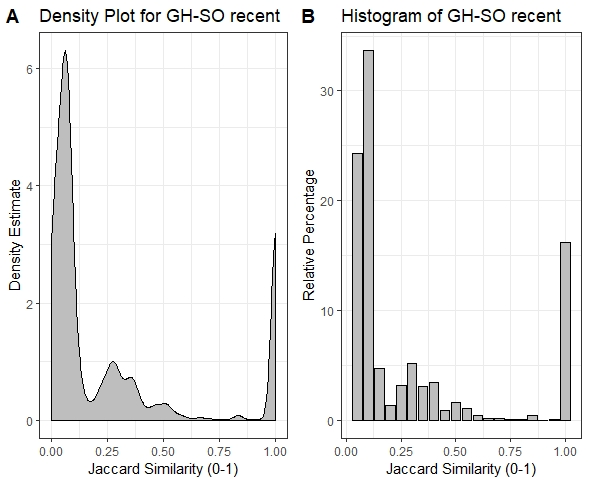
\includegraphics[width=\textwidth]{figures/GH_SO_recent.jpeg}\\
          \caption{Density Plot(A) and Histogram(B) of GH-recent and SO-recent data set comparison}
          \label{fig:GH_SO_recent}
        \end{figure}
        
        Figure \ref{fig:GH_SO_recent} and \ref{fig:overlap_GH_SO_recent} show the results of comparing the most recent activity of users on GitHub and Stack Overflow. For the rest of the analysis this will be referred to as the \emph{GH-recent - SO-recent} comparison. We chose \emph{Jaccard Similarity} as the similarity metric for this analysis, as we are interested in measuring the similarity between two sets of keywords for each user, coming from the \emph{GH-recent} and \emph{SO-recent} text corpora. Figure \ref{fig:GH_SO_recent} illustrates the distribution of the \emph{Jaccard Similarity} scores obtained from the \emph{GH-recent - SO-recent} comparison. Plot A shows a density plot, while Plot B is a  histogram of the \emph{Jaccard Similarity} scores. The distribution from Figure \ref{fig:GH_SO_recent} shows that the majority of the population has very low \emph{Jaccard Similarity} scores, which means that there is very low similarity between most user's \emph{GH-recent} and \emph{SO-recent} data. The histogram paints the most clear picture by showing that the highest relative percentage of \emph{Jaccard Similarity} scores are \{0, 0.05, 0.10 and 1\}.
        
        \begin{figure}
          % Requires 
          \centering
          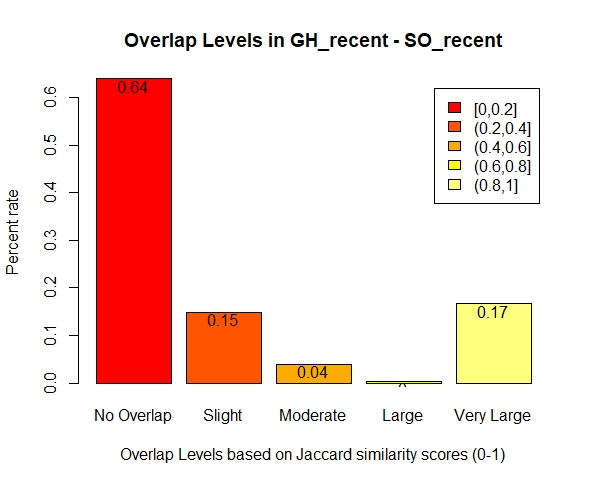
\includegraphics[width=\textwidth]{figures/overlap_GH_SO_recent.jpeg}\\
          \caption{Overlap levels between GH-recent and SO-recent data sets}
          \label{fig:overlap_GH_SO_recent}
        \end{figure}
        
         Figure \ref{fig:overlap_GH_SO_recent} drives home this point by creating five non-overlapping sub-intervals of \emph{Jaccard Similarity} scores from the [0,1] range, classifying each sub-interval of values to a scale of \emph{No, Slight, Moderate, Large and Very Large Overlap}. When comparing the GH-recent - SO-recent text corpora Figure \ref{fig:overlap_GH_SO_recent} clearly shows that 64\% of the population has no overlap, 15\% has slight overlap, 4\% has moderate overlap, and 17\% has a very large overlap. 
        
        \begin{figure}
          % Requires 
          \centering
          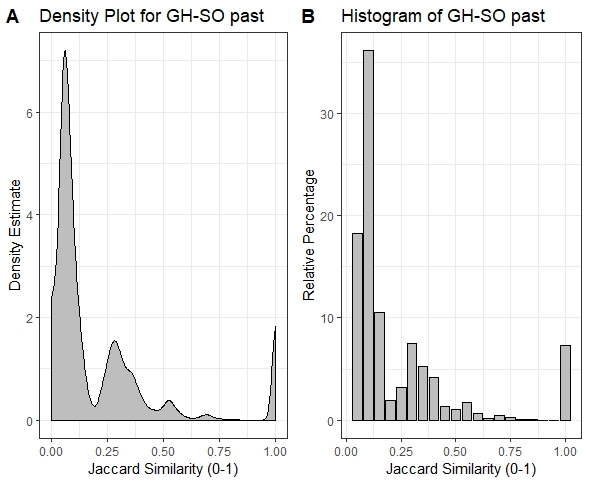
\includegraphics[width=\textwidth]{figures/GH_SO_past.jpeg}\\
          \caption{Density Plot(A) and Histogram(B) of GH-past and SO-past data set comparison}
          \label{fig:GH_SO_past}
        \end{figure}
        
        Figure \ref{fig:GH_SO_past} and \ref{fig:overlap_GH_SO_past} show the results of comparing the past activity of users on GitHub and Stack Overflow. This will be referred to as the \emph{GH-past - SO-past} comparison. Same as above, \emph{Jaccard Similarity} is the similarity metric chosen to measure the similarity between two sets of keywords for each user, coming from the \emph{GH-past} and \emph{SO-past} text corpora. Figure \ref{fig:GH_SO_past} illustrates the distribution of the \emph{Jaccard Similarity} scores obtained from the \emph{GH-past - SO-past} comparison. Plot A shows a density plot, while Plot B is a  histogram of the \emph{Jaccard Similarity} scores. The distribution from Figure \ref{fig:GH_SO_past} is similar to the one from Figure \ref{fig:GH_SO_recent} and it shows that the majority of the population has very low \emph{Jaccard Similarity} scores. The density plot shows that most of the population has \emph{Jaccard Similarity} scores of \{0.05, 0.10, 0.15\}, while there are quite a few extreme scores of 0 and 1. This distribution suggests that there is very low similarity between most user's expertise terms found in the \emph{GH-past} and \emph{SO-past} corpora. 
        
        \begin{figure}
          % Requires 
          \centering
          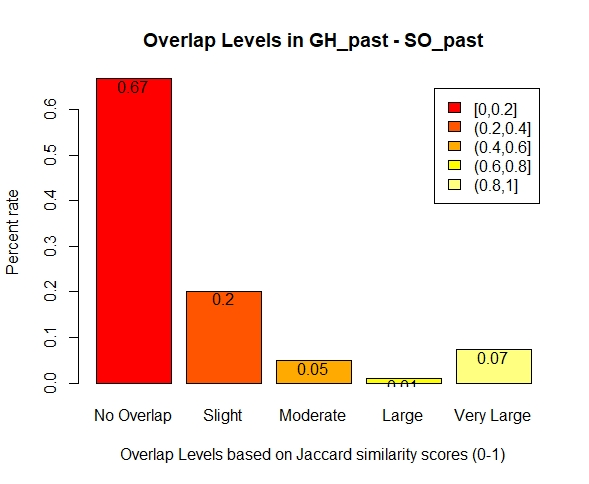
\includegraphics[width=\textwidth]{figures/overlap_SO_GH_past.jpeg}\\
          \caption{Overlap levels between GH-past and SO-past data sets}
          \label{fig:overlap_GH_SO_past}
        \end{figure}
        
        Figure \ref{fig:overlap_GH_SO_past} confirms the findings above by considering the same five overlap levels as in Figure \ref{fig:overlap_GH_SO_recent}. When comparing the expertise terms in the GH-past - SO-past text corpora Figure \ref{fig:overlap_GH_SO_past} shows that 67\% of the population has no overlap, 20\% has slight overlap, 5\% has moderate overlap, 1\% has large overlap, and 7\% has a very large overlap.
        
        \fbox{\begin{minipage}{\textwidth}
            Answer to RQ2: The comparison of GH-recent and SO-recent text corpora showed that 64\% of the population have no overlap, while the GH-past and SO-past comparison concluded that 67\% of the population have no overlap. These results suggest that the expertise developed by users on GitHub and Stack Overflow is mostly different.
        \end{minipage}}
    
    \section{Cross-platform Transferable Knowledge\label{sec:results_rq3}}
        % RQ3:  What knowledge is transferable from one platform to another?
        
        \begin{table}
          \centering
          \caption{Most common words in GH-past and SO-past data sets.}\label{tab:RQ3_past}
            \vspace{6pt} % Required to get proper spacing between caption and table
          \begin{tabular}{|c c c | c c c|}
            \hline
            Ranking & Keyword & Frequency & Ranking & Keyword & Frequency \\
            \hline\hline
            1 & library & 43123 & 16 & base & 16798 \\
            2 & code & 37621 & 17 & implementation & 16670 \\
            3 & simple & 32762 & 18 & client & 15833 \\
            4 & type & 30948 & 19 & test & 15723 \\
            5 & javascript & 30044 & 20 & http & 15674 \\
            6 & project & 26255 & 21 & page & 15423 \\
            7 & web & 25083 & 22 & game & 13890 \\
            8 & tool & 24967 & 23 & website & 13255 \\
            9 & https & 24738 & 24 & package & 12982 \\
            10 & file & 24737 & 25 & repository & 11690 \\
            11 & html & 22333 & 26 & add & 11421 \\
            12 & github & 21317 & 27 & method & 11421 \\
            13 & script & 20318 & 28 & line & 11252 \\
            14 & source & 20266 & 29 & api & 11144 \\
            15 & language & 19855 & 30 & datum & 10980 \\
            \hline
          \end{tabular}
        \end{table}
        
        
        \begin{table}
          \centering
          \caption{Most common words in GH-recent and SO-recent data sets.}\label{tab:RQ3_recent}
            \vspace{6pt} % Required to get proper spacing between caption and table
          \begin{tabular}{|c c c | c c c|}
            \hline
            Ranking & Keyword & Frequency & Ranking & Keyword & Frequency \\
            \hline\hline
            1 & test & 56302 & 16 & heroku & 15764 \\
            2 & simple & 51226 & 17 & buildpack & 15764 \\
            3 & library & 44781 & 18 & cli & 15764 \\
            4 & app & 43750 & 19 & rb & 15764 \\
            5 & api & 35881 & 20 & activerecord & 15764 \\
            6 & base & 26075 & 21 & rspec & 15764 \\
            7 & client & 25381 & 22 & active & 15764 \\
            8 & code & 22052 & 23 & github & 15297 \\
            9 & file & 21538 & 24 & web & 12890 \\
            10 & application & 19620 & 25 & add & 12849 \\
            11 & https & 16764 & 26 & change & 12849\\
            12 & ruby & 15764  & 27 & remove & 12849 \\
            13 & rail & 15764 & 28 & check & 12849\\
            14 & ember & 15764 & 29 & make & 11231 \\
            15 & gem & 15764 & 30 & comment & 11231\\
            \hline
          \end{tabular}
        \end{table}
        
        Co-occuring keywords: \textbf{test, simple, library, api, base, client, code, file, https, github, web} and \textbf{add}.
        
        \boxed{$Answer to RQ3:$}
    
    \section{Expertise Evolution\label{sec:results_rq4}}
        % RQ4: How does developer expertise evolve on Stack Overflow and GitHub?
                
        \begin{figure}
          % Requires 
          \centering
          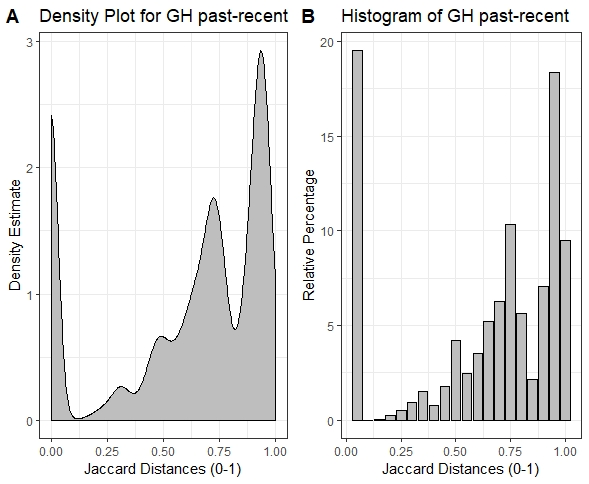
\includegraphics[width=\textwidth]{figures/GH_past-recent.jpeg}\\
          \caption{Density Plot(A) and Histogram(B) of GitHub past and recent data set comparison}
          \label{fig:GH_past_recent}
        \end{figure}
        
        \begin{figure}
          % Requires 
          \centering
          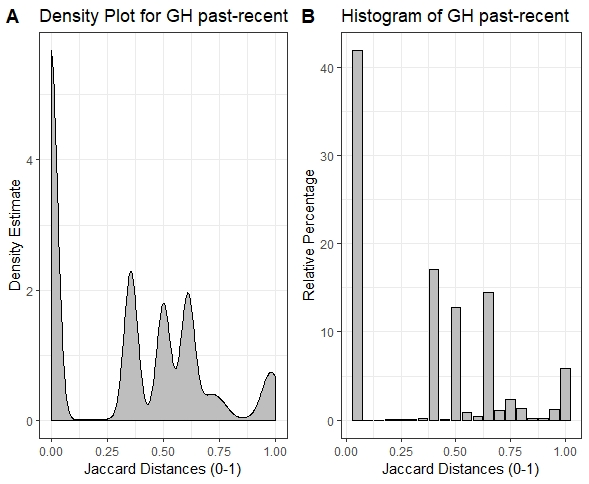
\includegraphics[width=\textwidth]{figures/SO_past-recent.jpeg}\\
          \caption{Density Plot(A) and Histogram(B) of Stack Overflow past and recent data set comparison}
          \label{fig:SO_past_recent}
        \end{figure}
        
        
        \begin{figure}
          % Requires 
          \centering
          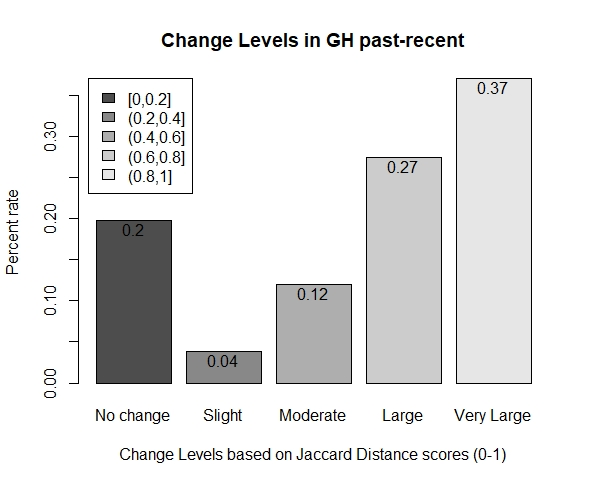
\includegraphics[width=\textwidth]{figures/change_level_GH_past-recent.jpeg}\\
          \caption{Change levels between GitHub past and recent data sets}
          \label{fig:change_GH_past_recent}
        \end{figure}
        
        \begin{figure}
          % Requires 
          \centering
          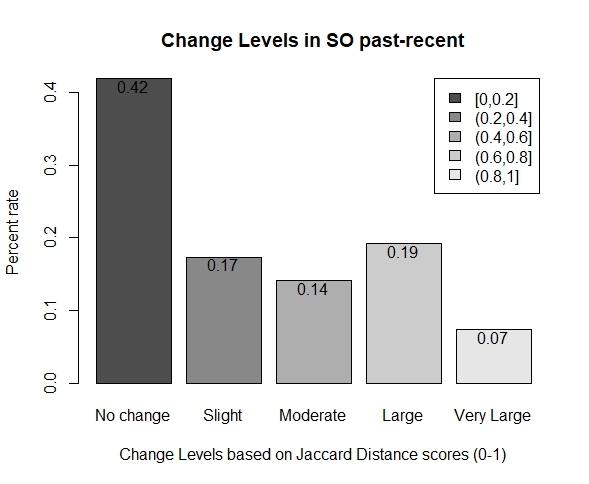
\includegraphics[width=\textwidth]{figures/change_levels_SO_past-recent.jpeg}\\
          \caption{Change levels between Stack Overflow past and recent data sets}
          \label{fig:change_SO_past_recent}
        \end{figure}
        
        \boxed{$Answer to RQ4:$}